\section{Обзор}
В данном разделе представлен обзор предметной области, включающий: общие 
сведения; способы реализации предметно-ориентированных языков вместе с
преимуществами и недостатками каждого из подходов; процесс отображения пользовательского интерфейсов в упрощённом виде; популярные языки
разработки мобильных приложений.

\subsection{Общие сведения}

\addtocontents{toc}{\protect\setcounter{tocdepth}{1}}

\subsubsection{Завершающие лямбда-выражения}
\label{section:trailing-lambdas}
\textit{Завершающие лямбда-выражения} (от англ. \textit{trailing lambdas})
--- синтаксические возможности некоторых языков программирования,
позволяющие при вызове функции, последним формальным параметром которой
является другая функция, передать в качестве последнего
аргумента лямбда-выражение, вынесенное за пределы синтаксического контекста
остальных аргументов. Добавление в язык завершающих лямбда-выражений
позволяет на уровне синтаксиса сделать неотличимыми конструкции языка
программирования и вызов вышеупомянутых функций.

На листинге~\ref{lst:antlr-trailing-lambda} представлен пример
синтаксического правила передачи завершающих лямбда-выражений, записанный
в нотации инструмента \name{ANTLR4}~\cite{antlr-homepage}.
\begin{lstlisting}[style=Antlr, caption=Синтаксическое правило завершающих
лямбда-выражений, label={lst:antlr-trailing-lambda}]
trailing_lambda
	: '{' parameters? (return_type 'in')? expression_sequence '}'
	;

function_call
	: function_name arguments? trailing_lambda?
	;
\end{lstlisting}
\subsubsection{Непрозрачные типы}
\label{section:opaque-types}
\textit{Непрозрачные типы} (от англ. \textit{opaque types})
--- механизм типовой системы языка программирования и его компилятора,
позволяющий функции или методу с непрозрачным типом возвращаемого значения
скрывать информацию о типе возвращаемого значения. Вместо того, чтобы
указывать конкретный тип в качестве типа возвращаемого значения функции,
тип возвращаемого значения описывается в терминах интерфейсов, которым
он соответствует. В отличие от возврата значения, тип которого является
типом интерфейса, непрозрачные типы сохраняют идентичность ---
компилятор имеет доступ к информации о конкретном типе, в то время как
клиенты функции или метода его не имеют.
%\subsubsection{\name{Accord}: спецификации}
%\label{section:accord-specs}
%Спецификации в языке \name{Accord} --- тип данных, являющийся именованным
%множеством сигнатур методов. Тип данных $T$ называется соответствующим
%спецификации $S$ тогда и только тогда, когда
%$SM \subseteq TM$, где $SM$ --- множество сигнатур методов спецификации $S$,
%$TM$ --- множество сигнатур методов типа $T$. Проверка на соответствие
%объекта определённого типа той или иной спецификации происходит во время
%выполнения программы за исключением случаев, когда данная проверка может
%быть проведена во время компиляции исходного кода с использованием
%статической информации о программе.

\addtocontents{toc}{\protect\setcounter{tocdepth}{3}}

\subsection{Предметная область}
\subsubsection{Предметно-ориентированные языки}
\label{dsl-section}
Предметно-ориентированный язык (\textit{domain-specific language}, DSL) ---
это язык программирования с более высоким уровнем абстракции,
отражающий специфику решаемых с его помощью задач. Такой язык оперирует
понятиями и правилами из определенной предметной области~\cite{book-of-dsls}.

В отличие от языков программирования общего назначения, таких как \name{C},
\name{Python}, \name{Java}, предметно-ориентированные языки предоставляют
абстракции, адекватные решаемой проблеме, позволяя выражать решения,
написанные с их помощью, кратко и ёмко; причём в некоторых случаях
использование DSL не требует квалификации программиста.
В качестве примера DSL можно привести \name{SQL} ---  декларативный язык
программирования, применяемый для создания, модификации и управления данными в
реляционной базе данных.
Основным недостатком применения предметно-ориентированных языков является
стоимость их разработки, требующая экспертизы как в области разработки языков
программирования, так и в целевой предметной области.
Это является одной из причин того, что предметные языки редко применяются
для решения задач программной инженерии, в отличие от языков программирования
общего назначения.
Другой причиной отказа от обособленных предметных языков является тот факт,
что сочетание программной библиотеки и языка программирования общего
назначения может заменять DSL.
Программный интерфейс (\textit{Application Programming Interface},
API) библиотеки содержит специфичный для определённой
области словарь, образованный именами классов, методов и функций, доступный
всем пользователям языков программирования общего назначения, подключившим
библиотеку.
Однако, вышеприведённый подход проигрывает предметным языкам в следующих
аспектах~\cite{when-and-how-develop-dsl,dsl-spectrum-wile}:
\begin{itemize}
	\item устоявшаяся в области нотация, как правило, выходит за рамки
	ограниченных механизмов определения пользовательских операторов,
	предоставляемых языками общего назначения;
	\item абстракции определённой области не всегда могут быть
	просто отображены в конструкции языков общего назначения~\cite{dsl-traversal-transform};
	\item использование предметно-ориентированного языка сохраняет
	возможность анализа, верификации, оптимизации, параллелизации и
	трансформации в рамках конкретной области, что, в случае работы с
	исходным текстом языка программирования общего назначения, является
	более сложной задачей.
\end{itemize}

\subsubsection{Подходы к реализации предметно-ориентированных языков}
В последнее время всё больше исследований в области
предметно-ориен\-тированных языков направлены на категоризацию предметных
языков, а также выработку советов и лучших практик, отвечающих на вопросы
"когда и как?" создавать DSL для конкретной области~\cite{when-and-how-develop-dsl,study-on-preliminary-approaches-develop-dsl,spinellis-dsl-patterns}.
\paragraph{Препроцессинг}
DSL-конструкции транслируются в более низкоуровневый программный код
базового языка программирования общего назначения.
\begin{itemize}
	\item \textit{Макрокоманда}. Конструкции предметного языка представлены
	символьными именами, заменяемыми при обработке препроцессором на
	последовательность программных инструкций базового языка.
	\item \textit{Транспиляция}. Исходный код предметного языка
	транслируется в исходный код языка общего назначения.
	\item \textit{Лексическая обработка}. Трансформация предметного языка в
	язык общего назначения осуществляется на уровне лексем.
\end{itemize}

Преимуществом данного подхода является простота реализации DSL, поскольку
большая часть семантического анализа выполняется средствами базового языка.
В то же время, это является и недостатком данного подхода ввиду отсутствия
предметно-ориентированного статического анализа, оптимизаций и сообщений об ошибках.

\paragraph{Встраивание в базовый язык}
В данном подходе конструкции базового языка используются для построения
библиотеки предметно-ориен\-тированных операций. С помощью синтаксиса
базового языка задаётся диалект, максимально приближенный к определённой
предметной области.

Преимуществом данного подхода является полное переиспользование компилятора или интерпретатора базового языка для построения DSL. Основными недостатками
являются сообщения об ошибках, соответствующие спецификации базового языка,
и ограниченная синтаксическая выразительность, обусловленная
существующим синтаксисом базового языка.

\paragraph{Самостоятельный компилятор}
В данном подходе для создания DSL используются методы построения
компиляторов или интерпретаторов. В случае компилятора, конструкции
предметного языка транслируются во внутреннее представление компилятора, а
статический анализ производится над спецификацией DSL. В случае
интерпретатора, конструкции предметного языка распознаются и выполняются
в ходе цикла выборки-распознавания-исполнения (от англ.
\textit{fetch-decode-execute cycle}).

Преимуществами данного подхода являются приближенные к предметной
области синтаксис языка и сообщения об ошибках. Серьёзным недостатком
является необходимость создания нового компилятора или интерпретатора
предметного языка.

\paragraph{Компилятор компиляторов}
Данный подход схож с предыдущим за исключением того, что все или некоторые
стадии компиляции выполняются с использованием \textit{компилятора компиляторов} --- программы, воспринимающей синтаксическое или семантическое
описание языка программирования и генерирующей компилятор для этого языка.

Преимуществом подхода является снижение расходов на создание компилятора
предметного языка. Ограниченность итогового DSL возможностями используемого
компилятора компиляторов, а также сложность проработки предметного языка в
деталях, что может быть критично для достижения определённого уровня
производительности и близости сообщений об ошибках к предметной области,
составляют недостатки данного подхода.

\paragraph{Расширение существующего компилятора}
Компилятор языка программирования общего назначения расширяется
предметно-ориенти\-рованными правилами оптимизации и/или генерации кода.

В сравнении с предыдущим, данный подход менее трудоёмок из-за возможности
переиспользования частей существующего компилятора. Однако, стоит отметить,
что расширение существующего компилятора может оказаться сложной задачей,
для выполнения которой необходима поддержка расширений со стороны
компилятора языка общего назначения, а также минимизация пересечений
синтаксиса и семантики базового и предметного языков.

\paragraph{Использование готовых инструментов}
Существующие инструменты и нотации адаптируются под конкретную предметную
область. Примером такого подхода являются DSL, основанные на нотации
\name{XML}. В большинстве случаев предметные языки, полученные данным
способом, плохо подходят для их использования людьми в ручном режиме.

\paragraph{Создание библиотеки функций}
В качестве предметного языка выступает язык программирования общего
назначения и библиотека функций, создающая своим интерфейсом словарь
предметной области.

Преимуществом подхода является его относительная простота, заключающаяся
в необходимости создания библиотеки функций предметной области. Недостатком
является сложность работы с таким языком для людей, не обладающими навыками
программирования.

\subsubsection{Отображение пользовательского интерфейса}
\label{section:render-pipeline}
В данном разделе описан процесс обновления пользовательского интерфейса,
ставший де-факто стандартом для популярных современных средств разработки
мобильных приложений. Стоит отметить, что далее будут рассмотрены лишь базовые принципы построения и отображения интерфейсов, которых должно быть
достаточно для объяснения тех или иных оптимизационных решений, принятых в
данной работе.

Задачей отображения пользовательского интерфейса занимается
так называемый движок рендеринга или отрисовки (\textit{ren\-dering engine})
--- программное обеспечение, генерирующее изображение по модели.
Здесь \textit{модель} --- это описание любых объектов или явлений на строго
определённом языке или в виде структуры данных.

Процесс отображения пользовательского интерфейса
(рис. \ref{render-pipeline}) состоит из последовательного построения
нескольких древовидных структур, каждая из которых является образом
графического интерфейса, записанного пользователем на некотором языке.
\begin{itemize}
	\item \textit{Дерево компонентов} --- древовидная структура данных,
	узлами которой являются	высокоуровневые представления графических
	компонент. Множество операций над деревом компонентов
	анализируется и оптимизируется, после чего применяется к дереву
	элементов, изменение которого является дорогостоящей операцией.
	Примером такого дерева может являться \name{VDOM}
	(от англ. \textit{Virtual Document Object Model} --- виртуальная
	объектная модель документа).
	\item \textit{Дерево элементов} --- древовидная структура данных,
	изоморфная дереву компонентов, элементы которой
	трансформируются в элементы дерева рендеринга для последующей
	их отрисовки графическим конвейером. В качестве примера такого дерева
	можно привести \name{DOM} (от англ. Document Object Model).
	\item \textit{Дерево рендеринга} --- древовидная структура данных,
	содержащая в себе только необходимую для отрисовки информацию.
	Элементами этого дерева являются базовые графические примитивы,
	доступные движку отрисовки.
\end{itemize}

При отрисовке следующего кадра, движок рендеринга перерисовывает только
изменившиеся по сравнению с предыдущим кадром части интерфейса. Для этого,
между двумя соседними кадрами находится разница, которая и отправляется в
движок отрисовки. Нахождение этой разницы является одной из наиболее
ресурсоёмких операций во время выполнения приложения, поскольку она требует
обхода дерева элементов интерфейса, нахождения узлов, соответствующих
потенциально изменяющимся компонентам графического интерфейса, сравнения
таких компонент текущего и предыдущего кадров.

\begin{figure}[H]
\centering
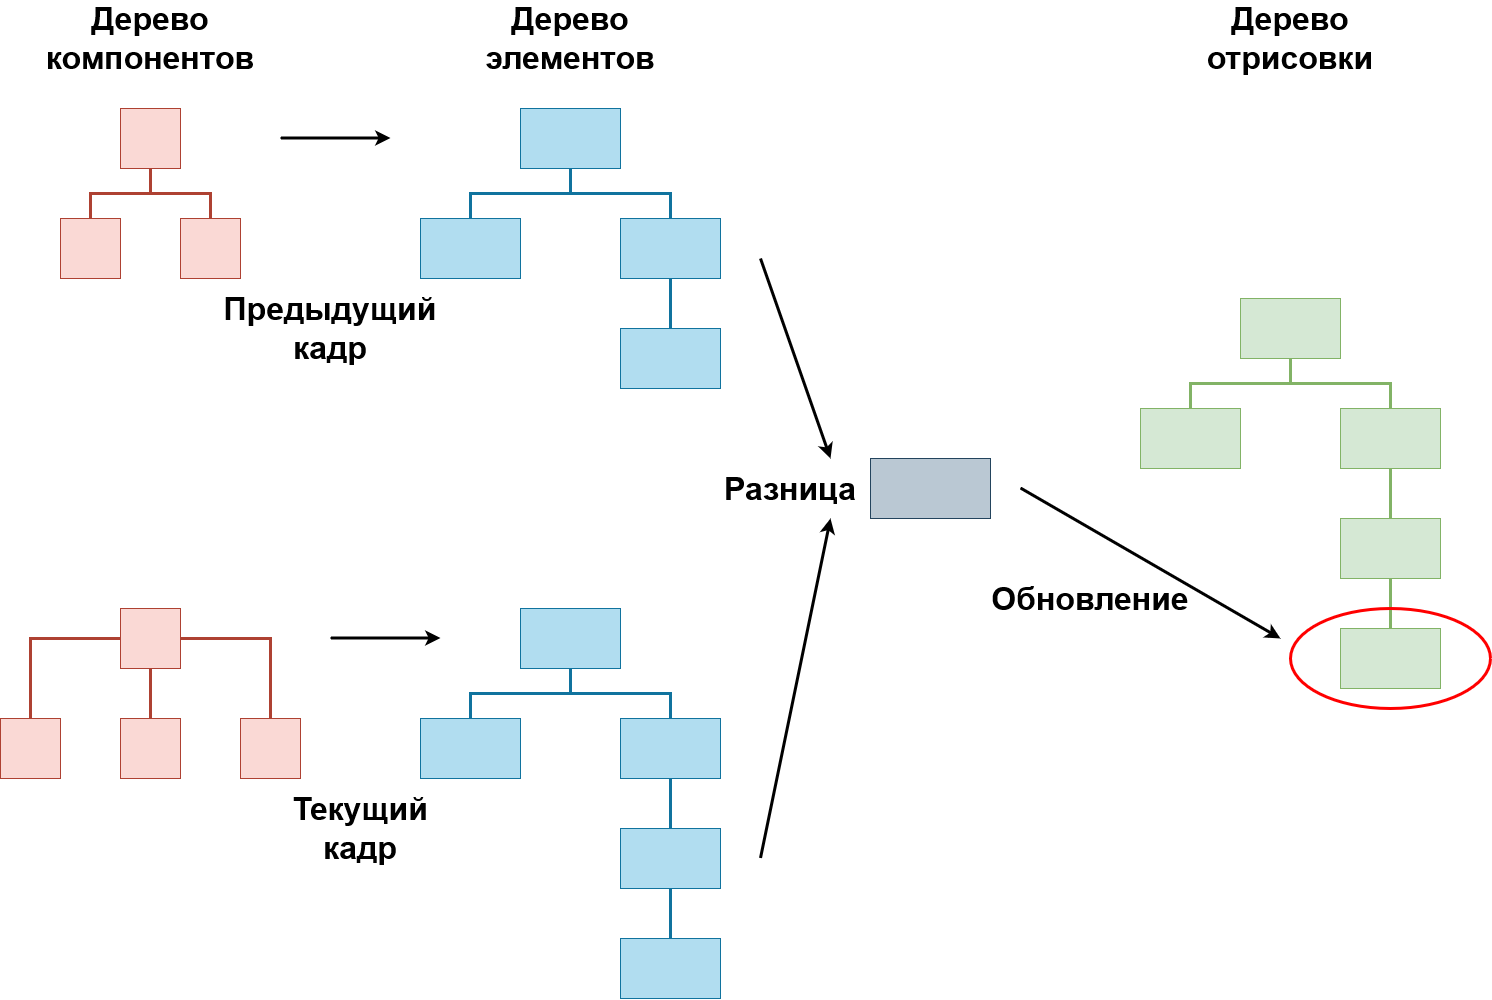
\includegraphics[width=\linewidth,height=0.9\linewidth,keepaspectratio]{resources/rendering-pipeline.png}
\caption{Процесс отображения пользовательского интерфейса}
\label{render-pipeline}
\end{figure}


\subsection{Существующие решения}
\subsubsection*{Dart / Flutter}
\name{Flutter}~\cite{flutter-homepage} --- язык разработки
мобильных приложений, представляющий из себя создающую словарь предметной
области библиотеку графических компонентов для языка
программирования общего назначения \name{Dart}~\cite{dart-homepage}.

На листинге \ref{lst:flutter-example} представлен пример исходного кода
приложения, написанного на языке \name{Flutter}.
Структура графического интерфейса описывается декларативно (строки 17-25).
Управление реактивными данными вынесено в отдельный
класс и осуществляется пользователем в явном виде: оборачивание всех
реактивных изменений в вызов специальной функции \textit{setState}, в
качестве аргумента которой передаётся лямбда-выражение, содержащее часть
бизнес-логики. При вызове этой функции, выполняется переданное ей
лямбда-выражение, после чего графическая компонента помечается как
компонента, требующая дальнейшего обновления.
\begin{lstlisting}[language=Swift,caption=\name{Flutter}. Счётчик нажатия кнопки,label={lst:flutter-example}]
class Counter extends StatefulWidget {
    Counter({Key key}) : super(key: key);
    
    @override
    _CounterState createState() => _CounterState();
}

class _CounterState extends State<Counter> {
    int _counter = 0;

    void _incrementCounter() {
        setState( () { _counter++; } );
    }
    
    @override
    Widget build(BuildContext context) {
        return Column(
            children: <Widget>[
                Text("Current count: $_counter"),
                TextButton(
                    onPressed: _incrementCounter,
                    child: Text("Click on me!")
                )
            ]
        )
    }
}
\end{lstlisting}

Отрисовка графического интерфейса средством разработки мобильных
приложений \name{Flutter} осуществляется по описанному в
пункте~\ref{section:render-pipeline} алгоритму.

\subsubsection*{Kotlin DSL / Jetpack Compose}
\name{Kotlin DSL} --- механизм языка \name{Kotlin}~\cite{kotlin-homepage},
позволяющий создавать на его основе предметно-ориентированные языки.
Завершающие лямбда-выражения~\ref{section:trailing-lambdas} и тот факт, что
результатом последовательности выражений является её последнее выражение,
суть основные техники, на основе которых реализован \name{Kotlin DSL}.

На листинге~\ref{lst:kotlin-example} представлен пример исходного кода
приложения, написанного с использованием фреймворка для разработки мобильных
приложений \name{Jet\-pack Compose}~\cite{jp-compose-homepage},
реализованного в виде надстройки над \name{Kotlin DSL}.
Структура графического интерфейса описывается декларативно (строки 5-10).
Управление реактивными данными скрыто от пользователя и не является частью
языка и компилятора. Работа с реактивными данными реализована в виде
библиотеки функций, например, \textit{remember} и \textit{mutableStateOf}
(строка 3).
\begin{lstlisting}[language=my_pseudo,caption=\name{Jetpack Compose}.
Счётчик нажатия кнопки,label={lst:kotlin-example}]
@Composable
fun Counter() {
    var count by remember { mutableStateOf(0) }
    
    Column() {
        Text(text = "Current count: ${count.value}")    
        Button(onClick = { count++ }) {
            Text(text = "Click on me!")
        }
    }
}
\end{lstlisting}

Отрисовка графического интерфейса любым средством разработки мобильных
приложений, построенным на базе \name{Kotlin DSL}, осуществляется по
описанному в пункте~\ref{section:render-pipeline} алгоритму.

\subsubsection*{JavaScript / React Native}
\name{React Native}~\cite{reactnative-homepage} --- фреймворк для разработки
мобильных приложений на языке программирования общего назначения
\name{JavaScript}. С точки зрения классификации предметно-ориентированных
языков, \name{React Native} является языком разработки мобильных приложений,
реализованным в виде библиотеки графических компонент.

На листинге~\ref{lst:react-example} представлен пример исходного кода
приложения, написанного с использованием фреймоворка \name{React Native}.
Структура графического интерфейса описывается в декларативном стиле
(строки 8-16).
Управление реактивными данным производится пользователем в явном виде:
все операции над реактивными данными оборачиваются в вызов предопределённой
функции \textit{setState}, которая по своему поведению аналогична такой же
функции в языке \name{Flutter}.
\begin{lstlisting}[language=my_pseudo,caption=\name{React Native}.
Счётчик нажатия кнопки,label={lst:react-example}]
class Counter extends React.Component {
  state = { count: 0 };

  incrementCounter = () => this.setState(
    prevState => ({ ...prevState, count: this.state.count + 1 })
  )

  render() {
    const { count } = this.state;
    return (
      <View>
        <Text>Current count: {count}</Text>
        <Button title="Click on me!" onPress={this.incrementCounter}/>
      </View>
    );
  }
}
\end{lstlisting}

Отрисовка графического интерфейса осуществляется по алгоритму, описанному в пункте~\ref{section:render-pipeline}.

\subsubsection*{Swift / SwiftUI}
\name{SwiftUI}~\cite{swiftui-homepage} --- язык разработки мобильных
приложений, реализованный методом встраивания в базовый
язык, которым, в данном случае, выступает язык программирования общего
назначения \name{Swift}~\cite{swift-homepage}.

На листинге~\ref{lst:swiftui-example} представлен пример исходного кода
приложения, написанного на языке \name{SwiftUI}.
Структура графического интерфейса описывается декларативно (строки 4-11). Реактивные данные помечаются пользователем декоратором \textit{@State}. Компилятор автоматически генерирует код, приводящий к обновлению графической компоненты в случае изменения реактивных данных.
\begin{lstlisting}[language=Swift,caption=Счётчик нажатия кнопки на языке
\name{Swift/SwiftUI},label={lst:swiftui-example}]
struct Counter : View {
    @State var count: Int = 0
	
    var body: some View {
        VStack {
            Text("Current count: \(count)")
            Button(action: { self.count += 1 }) {
                Text("Click on me!")
            }
        }
    }
}
\end{lstlisting}

С точки зрения синтаксиса, для достижения декларативности описания
интерфейса, в язык программирования \name{Swift} были добавлены следующие
возможности и языковые конструкции:
\begin{itemize}
	\item завершающие лямбда-выражения~\ref{section:trailing-lambdas};
	\item неявный возврат значений из функций, состоящих из единственного
	выражения возврата результата;
	\item непрозрачные типы
	(ключевое слово \textit{some})~\ref{section:opaque-types}
\end{itemize}

Особенностью \name{SwiftUI} является высокая степень использования
информации, доступной во время компиляции программы, для оптимизации
процесса отображения пользовательского интерфейса. Каждая графическая
компонента обладает статическим типом. Так, компонента \textit{Counter}
имеет следующий тип:
\begin{lstlisting}[escapeinside={(*}{*)}]
struct {
    count: Int
    body: VStack[Text, Button[Text]]
}
\end{lstlisting}
Зная тип каждой графической компоненты, процесс отображения интерфейса
может быть оптимизирован. Так, вместо алгоритма, описанного в
пункте~\ref{section:render-pipeline}, \name{SwiftUI} делает лишь точечные
вызовы обновления только тех компонент, которые могут потенциально
измениться во время работы приложения. Преимуществом такого подхода является
уменьшение потребления ресурсов процессора мобильным приложением во время
обновления кадра. При обновлении кадра пропадает необходимость в обходе
дерева компонент и проверки каждой компоненты на изменяемость.
Все оптимизированные процедуры обновления графических компонент генерируются
компилятором автоматически во время компиляции приложения. Как именно
\name{SwiftUI} использует статическую информацию о компонентах для
выполнения вышеописанной оптимизации неизвестно ввиду проприетарности и
закрытости данного решения.

%\subsubsection*{Вывод}
